\subsection{Theoretical comparison of general features} \label{section:featureanalysis}
The next step is to perform a theoretical comparison between the client-server model and the decentralized blockchain model. In this analysis the blockchain model is based on Ethereum, as it is used by another master thesis student, Axel Vallin, for implementation of another version of the system. This version is later compared to the centralized application, which was developed in this thesis work. The analysis considers both approaches from different perspectives and points of view in order to get better understanding about pros and cons, related to each approach, as well as the consequences with using them.

General trivia about Ethereum, which is quite important in order to grasp Ethereum and blockchain-related concepts, that are being touched upon in this analysis, is briefly described in the Appendix \ref{section:ether}. Readers, that are not familiar with Ethereum and blockchain networks in general, are strongly advised to read through the appendix before studying this analysis.

In order to get better picture from the economic perspective, Ether is typically converted to USD in the analysis. During the process of writing this thesis report, Ether price saw a couple of huge spikes and dips, which came at no surprise, knowing that Ether, along with other cryptocurrencies, is extremely volatile (as discussed in \ref{section:economics}). Therefore, for the purpose of consistency throughout the report, Ether price was assumed being equal to 700 USD. Usage of that rough approximation will be denoted with the star ($^\star$) notation in the report.

\subsubsection{Third party involvement and trust} \label{section:analysisthirdparty}
Trust is a sensitive subject in context of this study. Theoretically, usage of a decentralized blockchain, like Ethereum, is very much desirable from this point of view, as the third party involvement is completely eliminated by doing that. Centralized services, that are built using client-server architecture, are, in vast majority of cases, being maintained by some kind of third party organization. In this context, the term "third party" means an entity that is indirectly involved in an interaction between a set of users (typically a central authority). Having a third party that maintains control over the system, leads to all of the data being exposed to an indirectly involved entity, which in its turn implies that this entity has full control over the data (in most cases). This can be a potential source of a wide range of problems.

\paragraph{Identity frauds and data leaks}
Many of today's systems require users to provide their sensitive private information (such as their name, bank account number, address, job occupation, etc.), in order to function. This means that all of the data ends up being stored on the servers, which the user is not in control of. As the third party, that runs the service, has full control of these servers, as well as all of the data that is being stored on them, there is technically nothing that prevents the third party from misusing and exploiting that data for own purposes. Identity thefts are a very common type of crime nowadays. Once the criminals gain access to the sensitive private information, there is not much that can stop them from, for example, taking out a loan in victim's name, which can result in this victim being responsible for paying the loan back. According to Insurance Information Institute, the 2017 Identity Fraud Study found that 16 billion USD was stolen from 15.4 million U.S. consumers in 2016 \citep{idthefts}.

During the past decade, data exchange services like Dawex and BDEX has grown immensely. Anyone can register on these services and put a dataset up for sale. The big data exchange services have a policy of blocking all datasets that contain sensitive private information, but this can be avoided by encrypting the data, or by selling it through smaller services that does not have that policy. In theory, any company that uses a centralized ledger may extract all of the personal data and put it up for sale, by using an alias, to not disguise themselves.

\paragraph{Money frauds}
Some services have functionality of holding some of the user's money (like online casinos and such). In that case, users hand their money over to the third party, which maintains full control of those funds. If, for example, such company files for bankruptcy, users might find themselves left empty handed.

The original Blocket Secure Package fits into this category of services, as the money is stored in Blocket's account, during the merchandise transfer process. One can never be sure what Blocket does with the money until it is transferred to the seller. And, as mentioned before, there is also a theoretical possibility of Blocket seizing their operations and disappearing with the user's money.

\paragraph{Reputation of organizations and data protection laws}
Blocket is widely used by many people in Sweden, it has good reviews, which provides potential users with a belief, that the risk of getting scammed by Blocket is relatively low. However, there is a difference in considering that something is safe and something actually being safe. Regular users rarely get to know how their data is handled. In case of Blocket, there is some information to be found on their website about the guidelines, regarding handling of user data \citep{blocketuserdata}. However, there is no real 100\% guarantee that these guidelines are followed, as users do not have a possibility to check it in practice. In other words, users have to trust the company to follow the guidelines, regarding both handling of private data and assets. 

There are strict laws, regarding protection of personal data in developed and digitalized countries, such as Sweden, and companies are required to obey them. Regular checks and audits are performed to check if the companies are following the guidelines and terms of conditions. Thus, the terms of conditions, regarding the data handling on Blocket's website can be considered rather trustworthy. However, there are other less developed countries, where no such laws exist. Companies could then propose terms of conditions, just to trick users into believing that their data is safe and do whatever they want with it, without any risk of being punished. 

\paragraph{Fiat money}
Just about all public money these days is fiat money. Fiat money is typically issued by the government of a country. The government points to something and declares it being a bearer of monetary value. Might be a coin, might be a note, but the only reason it has value is because the government says so and makes people believe them. In that case, the government acts as a third party that is issuing the monetary assets, which can lead to some serious problems, as it did in Venezuela and Zimbabwe recently \citep{venezimbab}. This thesis work's topic is not about global economics, thus the reasons for potential problems are not discussed in detail. However, it is important to consider that any fiat currency has strong bonds to the issuing contry's politics. Bad political decisions may, and in fact will, reflect on the value of the currency, making it very volatile. Usage of digital asset token payment system, as proposed in the decentralized version of the service with no central governing body, eliminates that source of potential problems.
\subsubsection{Transparency} \label{section:transparency}

Some of the trust related issues, which are described in \ref{section:analysisthirdparty}, are caused by the mechanisms for data handling and system parameters being hidden from the users. Centralized systems do not typically reveal their code for public viewing. Data logs, parameters, transaction history, etc. can only be retrieved by the developers and system administrators. Thus, there is no possibility for regular users to check if the system is implemented to follow the guidelines, described in the terms of conditions (assuming that the user has some background and knowledge in software development and programming).

\paragraph{Transparency in blockchain} 
Many public blockchains, including Ethereum, which is used to build the decentralized Secure Package system, are transparent by default. This means that the entire blockchain is accessible by anyone. In case of Ethereum, an easy way to access and visualize the blockchain architecture behind it is to use a block explorer application, such as Etherscan \citep{etherscan}. All of the information about blocks, addresses/accounts (including smart contracts) and transactions is completely transparent and is viewable by using such a service.

\begin{figure}[H]
\centering
\includegraphics[scale=0.55]{images/etherscan.png}
\caption{Etherscan dashboard, showing recent blocks and transactions.}
\label{fig:etherscanrecent}
\end{figure}

As all of the transaction history is available, it is possible to see the amount of ETH that a given address/account is holding at the moment. Smart contract payload data and their corresponding source code can be viewed as well. In Ethereum, nothing is secret or hidden by default. This complete transparency results in numerous advantages, as well as a number of drawbacks, which are discussed later in this section.

\paragraph{Open source code management} 
Public blockchains are typically categorized as open source type of software. Unlike "closed source", or "proprietary" software, which is managed and controlled only by the person, team, or organization who created it (issues with that are briefly discussed in \ref{section:analysisthirdparty}), the source code of open source software can be inspected, modified, and enhanced by anyone that wishes to do so. In many cases, open source software is more desirable to use, as it typically gives more control to the users, can be used for training and learning, is more secure and is regularly tested by the community, which makes it more stable \citep{opensourceadvantages}.

Everything in Ethereum, including the website, tools, whitepapers and all of the software and compilers are 100\%, open source and is licensed under the GNU General Public License (GPL) \citep{gpl}. The code is constantly developed by the community, that dedicates resources and supports the project by contributing code to Ethereum's public repository \citep{ethereumrepo}. This makes the source code easily modifiable, very secure and thoroughly tested by the community and its administrators.

However, there is also a potential drawback, associated with open-source systems. There have been a few cases, when the bugs that were found in blockchain-based systems were exploited instead of being reported to the developers and fixed. Back in June 2016, the famous DAO hack was performed, by performing the recursive call exploit on the DAO token smart contract. A total of 3.6 million ETH was drained by the attacker within the first few hours of the attack. The aftermath of the DAO hack resulted in a lot of controversy within the Ethereum community \citep{dao}.

\paragraph{Issues with total transparency}
As mentioned before, all of the information, which is relevant to the network, is publicly accessible in Ethereum. This makes the network more trustworthy, as the information flow and transaction history, among other things, can be observed in detail. However, in some cases, like the one which is relevant for this study, namely the implementation of the Secure Package system, this results in some serious privacy-related issues. 

In order for the system to work, personal user data, such as names, addresses, contents of the package, recent GPS location of the package and other sensitive information needs to be stored in the smart contract and processed by the blockchain. There is no built-in data protection mechanisms in the network, thus making all of the personal data visible to the public. This is not desirable at all in context of Secure Package system, as without proper protection against the outsiders, this sensitive information may be used for identity frauds, as described in \ref{section:analysisthirdparty}.



\subsubsection{Data integrity, security and encryption} \label{section:analysisencryption}
It is very important that the user data is securely stored and is only viewable and modifiable by the actors, that are granted the permission. User data, which ends up being transparent by default when storing it on a blockchain, needs to be encrypted for privacy reasons, by using a robust cryptographic system. Communication channels between the front-end and the back-end (or a blockchain in case of the decentralized implementation) needs to be secure to prevent the intruders from intercepting the data, or perform a "man-in-the-middle attack". Apart from the "man-in-the-middle" attack, there are numerous other ways to hack a system, or tamper with its data. It is important to be aware of potential security risks, regarding each model of implementation. From the standpoint of data integrity and security, nothing comes close to being as good as a public blockchain.

\paragraph{Data persistence and integrity}
All of the data, that is added onto a public blockchain is immutable and cannot be removed. This is possible due to cryptographic bonds between the blocks in such a way, that a new block is indirectly connected to each of the previous blocks (i.e. new block's hash is dependent on the hash of the previous block, whose hash is dependent on its previous block's hash, etc.). Every block's hash is also dependent on the block's contents, which is defined by the merkle root of all the transactions, which are included in that particular block \citep{merkle}. Thus, even an insignificant change of a given block's contents affects all of the following blocks. This hostile change would easily be detected by the consensus protocol and discarded.

All of these features contribute towards blockchain being a near 100\% persistent data structure. The benefit of that data persistence is that the user can be sure about all of the information in a blockchain being verified and unchanged. This becomes rather important, when dealing with a network that supports digital assets, as this enables a trusted prevention of double spending problem and a trusted mechanism for the trace of payments. There is near to no risk regarding loss of data, as it is stored across multiple nodes and is cryptographically secured. The combination of blockchain's data integrity and absence of a third party results in a relatively high degree of trust.

When using a system with a database, the users may never be completely sure whether the data has not been tampered with by an intruder or an insider, which is related to the third party that runs and maintains the servers. This is the case because the data is typically not available for public audits and there, theoretically, is nothing that prevents the central organization, that is in control of the databases, from changing the values in the database fields. There are no cryptographic bonds between the entries in the tables, thus reducing the data persistence quality attribute, compared to blockchain based systems.

\paragraph{DDoS attacks}
Distributed denial-of-service attack, or \textit{\glspl{DDoS}}, is a cyber-attack, in which the attacker seeks to make a machine or network resource unavailable to its intended users by temporarily or indefinitely disrupting services of one or multiple hosts. Denial of service is typically accomplished by flooding the targeted machine or resource with requests in an attempt to overload systems and prevent some or all legitimate requests from being fulfilled \citep{ddos}.

DDoS attacks are experienced by the data centers in client-server oriented services on daily basis. Even though, the DDoS attacks are becoming more and more common and advanced, the protection systems are keeping up at a good pace. There are numerous data center protection solutions out there. Most protection services are using the approach of migrating data, during DDoS attacks, like the A10 Networks Thunder TPS Solution among others \citep{a10networks}. Services like Cloudfare are using advanced traffic filtering algorithms, along with data migration to achieve complete DDoS protection, as advertised on their website \citep{cloudfare}. It is very important to use proper DDoS protection for centralized applications in order to minimize risks of downtime.

When dealing with Ethereum, there are built in mechanisms to directly and indirectly provide DDoS protection. A recepie for a successful DDoS attack is to create congenstion rate greater than, or close to the network's maximum throughput. Ethereum's throughput is defined by block gas limit and target block time, as described in \ref{section:scalability}. During a DDoS attack the gas limit of the new blocks would quickly be reached, thus increasing the pool of pending transactions that are awaiting confirmation. As the frequency of new block addition is kept the same at approximately 15 seconds, an attacker could theoretically send a lot of transactions, fill every block with them and quickly overflow the network. Technically, this would be rather easy to achieve. However, each and every transaction consumes gas, which has to be paid for (see Section \ref{section:economics}). Thus, the attacker would have to pay for each individual DDoS transaction. It is possible to pay 0 Gwei for gas, however, these transactions would not be prioritized by miners, thus making it impossible to create a DDoS attack with them. In order to occupy nearly all of the throughput, the attacker needs to assign high gas prices, which would result in the hostile DDoS transactions being prioritized over regular transactions, that have lower gas limit. The cost of performing a DDoS attack is described in following equation:

\begin{align}
C_{\mathrm{att}} &= Q_{\mathrm{gas}}  \cdot C_{\mathrm{Gwei}} \cdot T_{\mathrm{net}} \cdot P_{\mathrm{att}} = Q_{\mathrm{gas}}  \cdot C_{\mathrm{Gwei}} \cdot \frac{L_b}{t_b} \cdot P_{\mathrm{att}}
\end{align}

Here, $T_{\mathrm{net}}$ is Ethereum's network throughput, defined by Equation (\ref{eq:eththroughput}). The block time $t_b$ is 15 seconds, or 1/240 hours. Gas price $C_{\mathrm{gas}}$ is the gas price chosen by the attacker, $C_{\mathrm{Gwei}}$ is current price of one Gwei ($10^{-9}$ ETH) in terms of fiat currency. Gas block limit $L_{b}$ is equal to approximately $8 \cdot 10^6$ gas at the time of writing. Percentage of hostile transactions $P_{\mathrm{att}}$ is a measure of total desired hostile congestion rate of the attack (0.8 means that 80\% of the transactions in each block are hostile), assuming that nearly all other transactions have lower gas limit than the corresponding $C_{\mathrm{gas}}$. This yields a linear function for the cost of attack $C_{\mathrm{att}}$:

\begin{align} \label{eq_1}
C_{\mathrm{att}} &\approx C_{\mathrm{gas}}  \cdot 10^{-9} \cdot C_{\mathrm{Gwei}} \cdot 8 \cdot 10^{6} \cdot 240 \cdot P_{\mathrm{att}}\\
C_{\mathrm{att}} &\approx 1.92 \cdot C_{\mathrm{gas}}  \cdot  C_{ETH} \cdot P_{\mathrm{att}}
\end{align}

\begin{figure}[H]
\centering
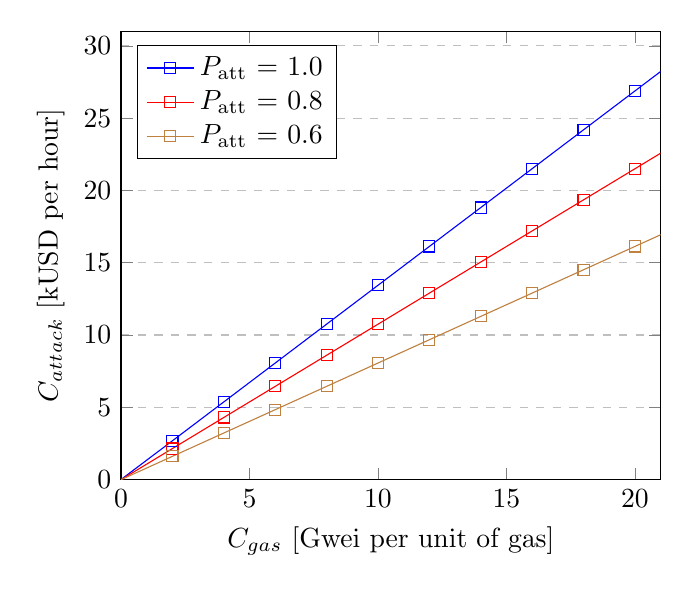
\begin{tikzpicture}
\begin{axis}[
    xlabel={$C_{gas}$ [Gwei per unit of gas]},
    ylabel={$C_{attack}$ [kUSD per hour]},
    xmin=0, xmax=21,
    ymin=0, ymax=31,
    xtick={0,5, 10, 15, 20},
    ytick={0, 5, 10, 15, 20, 25, 30},
    legend pos=north west,
    ymajorgrids=true,
    grid style=dashed,
]
 
\addplot[
    color=blue,
    mark=square,
    ]
    coordinates {
    (-2,-2.668)(2,2.688)(4,5.376)(6,8.064)(8,10.752)(10,13.440)(12,16.128)(14,18.816)(16,21.504)(18,24.192)(20,26.880)(22,29.568)
    };
    
\addplot[
    color=red,
    mark=square,
    ]
    coordinates {
    (-2,-2.150)(2,2.150)(4,4.300)(6,6.450)(8,8.600)(10,10.750)(12,12.900)(14,15.050)(16,17.200)(18,19.350)(20,21.500)(22,23.650)
    };
    
\addplot[
    color=brown,
    mark=square,
    ]
    coordinates {
    (-2,-1.612)(2,1.612)(4,3.226)(6,4.838)(8,6.451)(10,8.064)(12,9.676)(14,11.289)(16,12.902)(18,14.515)(20,16.128)(22,17.741)
    };
    \legend{$P_{\mathrm{att}}$ = 1.0, $P_{\mathrm{att}}$ = 0.8, $P_{\mathrm{att}}$ = 0.6}
 
\end{axis}
\end{tikzpicture}
\caption{Hourly cost of a theoretical DDoS attack in thousands of USD.}
\label{fig:ethddos}
\end{figure}

As can be seen in Figure \ref{fig:ethddos}, even when the attacker pays only 2 Gwei for single unit of gas and desires to establish a 60\% reduction of throughput (which would not harm the Ethereum network significantly at current state) by generating hostile transactions, it would come at a cost of approximately 2.30 ETH, or 1612 USD$^\star$ per hour. Gas price of 2 Gwei is considered to be a standard price at the time of writing. It is used in transactions for confirmations times of around few minutes, when network is moderately congested. As mentioned before, attackers would need to use a much higher gas price to block the significant part of network's throughput. A more realistic figure to look at would be gas price of around 10-15 Gwei and $P_{\mathrm{att}}$ of 0.8. An hour of such an attack would cost tens of thousands of dollars to perform. Even if the attack is performed using transactions with high gas price $N$, regular users would still be able to generate transactions and get them added to new blocks by simply using gas price of $\geq N$, which is larger then the DDoS transactions' gas price.

One more thing to consider, regarding DDoS attacks on Ethereum, is that the gas block limit is gradually increasing, as the total network hashpower grows. Recent increase from approximately $6.7 \cdot 10^6$ to around $8 \cdot 10^6$ gas happened in December 2018. Further growth of block gas limit would make theoretical DDoS attacks even more expensive, as it would lead to increased throughput of the network.

\paragraph{51\% attacks}
One of the most common potential threats to public blockchain-based systems are the \textit{\glspl{51 attack}}. The consensus principal in most blockchain based systems is indeed very much the same, as how the presidential elections in democratic countries are held, namely that the candidates need to gain the majority of votes, in order to be elected. The same principal is applied in nearly all public blockchains. In order for a new block to be added, it has to be accepted by the majority of nodes. Thus, 51\% attack refers to an attack on a blockchain by a group of miners controlling more than 50\% of the network's mining hashrate, or computing power. The possession of a total hashrate percentage of over 50\% would result in potential attackers being able to prevent new transactions from gaining confirmations, allowing them to halt payments between some or all users. They would also be able to reverse transactions that were completed while they were in control of the network, meaning they could double-spend digital assets. However, if such an attack was to take place, the attackers would still be unable to change the contents of previous blocks or generate new coins and tokens in cryptocurrency-related blockchains.

In case of Ethereum, such an attack would be possible, but highly unlikely to happen. Mining in general is such a popular activity nowadays, making Ethereum's hashrate relatively high, as shown in Figure \ref{fig:ethereumhashrate}. Therefore, the possession of more that 50\% of Ethereum's hashrate by a single person or organization is very unlikely, as it requires enormous resources. However, this enormous popularity and huge hashrate of Ethereum has resulted in solo mining being no longer viable, as the time to confirm a block by mining solo is often measured in months, or even years in case of some popular networks, depending on the size of mining operation and luck factor. This led to the introduction of, so called, \textit{\gls{pool mining}}. Its concept is that the miners join a pool, which distributes nonces to different mining subnodes (in other words, miners are cooperating between eachother to find blocks, when pool mining). Miners then get a share of total block reward from the blocks that have been found by the pool. This basically means that the mining pool is being in the possession of all the contributed hash power. This can lead to security concerns if the pool's total hashrate becomes more than a half of the total network hashrate, as it enables the pool to execute such 51\% attack.

\begin{figure}[H]
\centering
\includegraphics[scale=0.49]{images/ethereumhashrate.png}
\caption{Overall Ethereum network hashrate \textnormal{\citep{ethhashrate}}.}
\label{fig:ethereumhashrate}
\end{figure}

However, hitting 51\% network control is not a guarantee of success, it is just the point where success is likely. In fact, a node could attempt this sort of attack with much less network control, but the odds of success would be very low \citep{51perattack}. 

There is an obvious conclusion that can be drawn, regarding the 51\% attacks. Network's exposure to such attacks proportionally decreases, when the overall network hashrate increases. Smaller blockchain networks are obviously more exposed to 51\% attacks, than larger, more popular networks, that possess higher hashrates.

\paragraph{Man-in-the-middle attacks}
A \textit{\gls{man-in-the-middle attack}} is a type of cyberattack, in which a malicious actor inserts him/herself into a conversation between two parties, impersonates both parties and gains access to information that the two parties were trying to send to each other. In case of such attack, a malicious actor may try to intercept, send and receive data meant for someone else, or not meant to be sent at all, without either outside party knowing until it is too late \citep{mitm}.

Any system, that communicates via the Internet is exposed to such attacks. Thus, the communication channel between the user and the service, whether it is a blockchain or a server, has to be secure. A common technique, which is used in order to achieve that is digital signatures. Digital signatures ensure that the contents of the message, which was transmitted through the channel, were not tampered with, or changed.

\paragraph{Smart contracts and security flaws}
Ethereum is an extremely secure network. As was discussed before, it has a sufficient enough protection against 51\% attacks and DDoS attacks are extremely costly and impractical to perform. However, it is still possible to implement buggy smart contracts, that would introduce potential security flaws. The DAO hack, which was briefly mentioned in \ref{section:transparency}, happened due to that particular reason, as there was a bug in the DAO smart contract, which was discovered by the attacker and exploited. Thus, the developers need to be extremely careful, during the implementation process, in order to prevent such events from happening. A tool, which might be useful for that purpose is called Oyente. This tool can be used to test the smart contract code for bugs and security breaches \citep{oyente}.

\paragraph{Encryption in centralized systems}
There are many cryptographic solutions that can be chosen for the implementation of centralized systems. There are countless different algorithms out there, that are typically using two main cryptographic approaches: symmetric and asymmetric.

\textit{\Gls{symmetric encryption}} is the simplest kind of encryption that involves only one secret key to cipher and decipher information. Symmetrical encryption is an old and best-known technique. It uses a secret key that can either be a number, a word or a string of random letters. It is a blended with the plaintext of a message to change the content in a particular way. The sender and the recipient should know the secret key that is used to encrypt and decrypt all the messages. Blowfish, AES, RC4, DES, RC5, and RC6 are examples of symmetric encryption. The most widely used symmetric algorithm is AES-128, AES-192, and AES-256. The old and outdated DES algorithm is now used in a 3DES configuration, which basically involves execution of DES three times. The main disadvantage of the symmetric key encryption is that all parties involved have to exchange the key used to encrypt the data before they can decrypt it.

\textit{\Gls{asymmetric encryption}} is also known as public key cryptography, which is a relatively new method, compared to symmetric encryption. Asymmetric encryption uses two keys to encrypt a plaintext. It is important to note that anyone with a secret key can decrypt the message and this is why asymmetrical encryption uses two related keys to boosting security. A public key is made freely available to anyone, while private key is kept a secret. A message that is encrypted using a public key can only be decrypted using a private key, while also, a message encrypted using a private key can be decrypted using a public key. Security of the public key is not required because it is publicly available and can be passed over the Internet. Asymmetric key has a far better power in ensuring the security of information transmitted during communication. Asymmetric encryption is mostly used in day-to-day communication channels, especially over the Internet. Popular asymmetric key encryption algorithm includes RSA, DSA, Elliptic Curve (used in Ethereum and many other blockchains), PCKS and others \citep{pubvssym}.

\begin{figure}[H]
\centering
\includegraphics[scale=0.55]{images/pubpriv.png}
\caption{Public key cryptography (A) and symmetric encryption (B) illustrations.}
\label{fig:keygenerationether}
\end{figure}

Different encryption algorithms are good in different aspects and bad in other ones. For example, symmetric encryption algorithms are significantly faster than the asymmetric ones, however, they involve transmission of private keys before the communication can take place, thus introducing a risk of private key being intercepted. It is important to use encryption algorithms that are right for the task at hand.

\paragraph{Possible encryption mechanism in smart contracts}
Theoretically, the smart contracts can easily store 256-bit application-specific public keys of addresses, using data structure, called \texttt{mapping}. It maps key value pairs, where the keys could potentially correspond to users' Ethereum addresses and the values could correspond to the application-specific public keys. As mentioned in \ref{section:transparency}, Ethereum is completely transparent, thus the sensitive private information of users in the blockchain based Secure Package system would be exposed to the public, if not encrypted. 

The solution for that could be to generate individual Secure Package key pairs off-chain, store private keys securely at the user's computer and upload public keys to corresponding mappings inside of the smart contract. The reason behind generation of keys off the chain is that it prevents serious security and efficiency issues with on-chain generation.

Thus, it is theoretically possible to create encryption protocols for data transfer and storage in Ethereum. The keys would need to be 256-bit long, while still being able to provide secure encryption that can withstand hostile intrusion attacks. This can be achieved with elliptic curve cryptography in rather the same manner, as how Ethereum addresses' key pairs are generated. This is covered in greater detail in the next paragraph.

\paragraph{Key distribution and generation in Ethereum}
Public key cryptography is widely used in blockchain-based systems. Private keys are used to sign the transactions and generate public keys. As mentioned before, the Ethereum blockchain is completely transparent. This makes generation and distribution of private keys on-chain a very bad idea, as the keys can be intercepted by anyone, thus making them useless.

To solve these issues, the private key generation process for new Ethereum accounts is performed off-chain by taking any random 256-bit number and storing it safely off-chain. This 256-bit number acts as a private key. Public key is then generated from that random private key, which in its turn generates the account address. Key pairs are used for verification purposes and the address is used for indexing.

\begin{figure}[H]
\centering
\includegraphics[scale=0.62]{images/ethaddr.png}
\caption{Generation of keys and addresses in Ethereum. Private key is stored off-chain. Generation process involves the ECDSA algorithm, along with Keccak256 hashing algorithm \textnormal{\citep{ethyellow}}.}
\label{fig:keygenerationether}
\end{figure}

Using this approach, the private key is never being sent over the blockchain. This makes it very difficult for the intruder to access the account, assuming that a properly chosen seed has been used to randomly generate the private key. The are theoretically only two ways to break such 256-bit ECDSA private key. The first and most straightforward way would be to try all of the possible key combinations, which might take billions of years with the current technology, as there are $2^{256}$ possible keys. This approach is often referred to as "brute force". The second way is to solve the Elliptic Curve Discrete Logarithm Problem (ECDLP), which the ECDSA algorithm is based on. Rough estimates of solving this problem by using raw processor power is around $38.5 \cdot 10^{20}$ years, assuming that the encryption has been done properly and that private key possesses high degree of randomness. There are other approaches to solving this problem, by exploiting mathematical properties, such as hyperelliptic curves and elliptic curves with small complex multiplication fields \citep{ecdsa}.

Ethereum's public key cryptography, which is based on ECDSA, is considered being very secure, despite using rather short key size, compared to RSA, in which key lengths of up to 4096 bits are used \citep{rsakeys}. This has to do with the complexity of underlying mathematical problem. The mathematical problem that RSA is based on is prime number factorization, which is a lot less complex than ECDLP. That is the reason for a rather short key size in ECDSA.

Nevertheless, as long as the private key file is securely stored on the user's computer, there is little to no risk of the account being broken by an intruder.

\subsubsection{Scalability, performance and constraints} \label{section:scalability}

\paragraph{Availability and downtime}
Some client-server systems are very vulnerable to server breakdowns, as they, in many cases, drastically reduce service's bandwidth, or make the service stop working altogether. High availability and low downtime is a must for a highly congested client-server architecture. These factors are strongly dependent on the server infrastructure, its degree of decentralization, integration of data migration tools and possesion of back-up servers. Ethereum, however, possesses high degree of availability, due to its decentralized nature. If one of the nodes fail, there are still plenty of other nodes available.

\paragraph{Unpredicted confirmation delay}
When dealing with blockchain based systems, it is important to consider that a newly generated transaction has to be added to a block, before being confirmed and validated. This process may take different amounts of time, depending on the network's current state and network's target block time. Ethereum's target block time of 15 seconds is quite short, comparing to other blockchains like ZCash and Bitcoin, whose block times are 2.5 and 10 minutes respectively. However, even if a transaction is included into the blockchain's next block by the miners, the data will not become a part of the blockchain until the block has been mined. Target block time does not provide any guarantee that the block will be added to the chain within the target time, as the mining process itself involves a degree of randomness. Thus, the block finding time is heavily dependent on luck factor and is impossible to predict. A test, in which actual block times of 10000 blocks of Ethereum are analyzed can be found in Figure \ref{fig:ethtimetest} of Appendix \ref{section:blocktimes}.

There is as well no guarantee on the number of new blocks being found before the generated transaction itself will be included into a new block. This is heavily dependent on the gas price, which is chosen for the transaction. In applications that need to perform a large number of smart contract function calls, there is a trade-off to be made between the cost and latency, as faster response times will be a lot more expensive to achieve (detailed discussion about that is provided in \ref{section:economics}).

Introduction of such delay makes the implementation of applications, in which the responsiveness is a key factor, impossible. Such example is applications for real time monitoring. In some systems it is crucial to be notified about a problem, or a system state change as soon as possible. By using Ethereum to power such application, operators in the control room would not be notified about, for example, a potential problem which generates an alarm, before the transaction, that was generated by the alarm contract, was mined (which, as explained before can be take indefinite amount time). In such systems it is much more viable to use client-server architecture-based alarm system.

\paragraph{Ethereum's throughput and scalability} 
One of the main things to consider, when talking about a system's performance, is its maximum throughput and how it can be increased when needed. In Ethereum, the maximum throughput of the network is defined by the gas limit of the blocks and their frequency, using the following formula:

\begin{equation} \label{eq:eththroughput}
T_{\mathrm{net}} = \frac{1}{t_b} \cdot L_b = \frac{L_b}{t_b}
\end{equation}

Ethereum's block time $t_b$ is equal to 15 seconds, which can be converted to 1/240 hours. Block gas limit is equal to $8 \cdot 10^6$ at the time of writing. This block gas limit $L_b$ can be changed by miners, depending on overall network hashrate and congestion. Thus, by inserting the values into Equation (\ref{eq:eththroughput}), the current total throughput rate of Ethereum, $T_{\mathrm{net}}$, is approximately $1.6 \cdot 10^9$ gas/hour.

A basic Ethereum transaction for token transfer consumes 21000 gas, thus the current theoretical transaction capacity of Ethereum is approximately 76200 tx/h, assuming that none of the contracts executes any code. The theoretical transaction capacity is significantly reduced, when introducing transactions that require computational effort. 

The block gas limit has historically been increasing as a result of the growing hashrate of Ethereum network. The main reason for the existence of gas limit is to enable consensus participation of smaller mining nodes, thus further decentralizing the network. All of the transactions and their associated code has to be verified by the nodes. So without a proper limit on amount of gas per block, the nodes could potentially be overwhelmed. 

As mentioned earlier, increased congestion of the network can be addressed by adjusting the block gas limit $L_b$. The result of that gas limit would lead to a proportional increase in throughput in terms of gas, according to Equation (\ref{eq:eththroughput}).

\begin{figure}[H]
\centering
\includegraphics[scale=0.49]{images/gasblocklimit.png}
\caption{Gas block limit increase. Limit has been increased by four times since October 2016 to accommodate the growing congestion \textnormal{\citep{ethgaslimit}}.}
\label{fig:ethergasblocklimit}
\end{figure}

Nevertheless, despite the throughput's flexibility, which is provided by the gas block limit adjustment, it would be wrong to say that Ethereum possesses good scalability, as its theoretical average throughput of around 21 transactions per second is extremely poor, in comparison to typical client-server systems. The throughput needs to be scaled by an extremely large factor, in order for Ethereum network to possess comparable throughput to a typical client-server system, which can not be achieved fast enough by just increasing the gas block limit alone. 

\paragraph{Storage and memory}
Each and every smart contract has its own independent storage. That storage is virtual and is structured in terms of indexable key-value pairs. There are $2^{256}$ key-value pairs in each contract, with each pair having a capacity of storing 32 byte words, that results in a storage capacity of $2^{261}$ bytes. Thus, there is no doubt that there is plenty of storage, which is an understatement (as it turns out, a single smart contract has a theoretical capacity to store all of the humanity's data billions and billions times over).

This all sounds really good on paper, however, there is a cost that comes with using this storage. Storing a single 256-bit word consumes 20000 gas ({\small SSTORE} operation when the value is altered from zero to non-zero), excluding the base transaction cost of 21000 gas. In order to upload large files to smart contracts, they would need to be broken down to small 256-bit chunks and stored in different key-value pairs, using {\small SSTORE}. Equation (\ref{eq:filestorage}) derives the cost of storing a file in a smart contract.

\begin{align} \label{eq:filestorage}
C_{\mathrm{store}} = C_{\mathrm{gas}}\left(\frac{Q \cdot G_{sstore}}{256} + G_{tx}\right) \cdot 10^{-9} \cdot C_{ETH}  
\end{align}

Here, $Q$ is the file size. The file size is given in megabytes (1 megabyte is equal to $8 \cdot 10^6$ bits). Gas consumption of a single {\small SSTORE} operation, $G_{\mathrm{sstore}}$, is 20000. Base transaction cost, $G_{\mathrm{tx}}$, is 21000. Assuming that a gas price, $C_{\mathrm{gas}}$, of 2 Gwei was used, the following equation is derived.

\begin{align}
C_{\mathrm{store}} &= 2 \cdot \left(\frac{8 \cdot 10^6 \cdot 20000 \cdot Q}{256} + 21000\right) \cdot 10^{-9} \cdot C_{ETH} \approx 1.25 \cdot C_{ETH} \cdot Q
\end{align}

Thus, a single megabyte of storage costs approximately 1.25 ETH, or 875 USD! That is an exceptionally high price to pay, considering that services like Dropbox offer cloud storage of 2 terabytes at a monthly cost of around 12 USD \citep{dropbox}.

Another limitation on storage of large files in smart contracts is the gas block limit $L_b$. A transaction may obviously not exceed the gas block limit, as it would be impossible for it to be included in a block otherwise. Considering the current block gas limit of $8 \cdot 10^6$, the theoretical maximum amount of {\small SSTORE} operations triggered within a single transaction is derived using following equation.

\begin{align}
N_{sstore} = \floor[\Bigg]{\frac{\left(L_b - G_{tx} \right)}{G_{sstore}}} = \floor[\Bigg]{\frac{\left(8 \cdot 10^6 - 21000\right)}{20000}} = 389
\end{align}

Thus, there will be an overhead of 21000 gas approximately each 389 {\small SSTORE} operations (which corresponds to storage of 99584 bits). Equation (\ref{eq:filestorage}) needs to be modified with that overhead in mind.

\begin{align} \label{eq:newstorecost}
C_{\mathrm{store}} = C_{\mathrm{gas}}\left(\frac{Q \cdot G_{sstore}}{256} + G_{tx}\left(\frac{Q}{256}\middle/\floor[\Bigg]{\frac{\left(L_b - G_{tx} \right)}{G_{sstore}}}\right)\right) \cdot 10^{-9} \cdot C_{ETH} 
\end{align}

By numerically solving (\ref{eq:newstorecost}), the cost of storage turns out to be equal to approximately 1.266 ETH, or 886.20 USD$^\star$ per megabyte.

Additional consequence of splitting the file storage process into multiple transactions, spanning multiple blocks, is that the upload might take a long time, as the target block time is around 15 seconds. Assuming that each and every following block is filled with file content upload transactions until the storage process is completed, the average transmission speed would be 99.6 kilobits every 15 seconds, which translates into roughly 6.6 kilobits second. Even the dial up modems from the 90s had faster speeds of around 56 kilobits per second \citep{dialup}. At that rate the storage process of one megabyte would span over 81 blocks, thus taking approximately 20.25 minutes to complete, assuming that no other transactions are being included in any of those 81 blocks (but the last one), which is very unlikely.

However, once the data is added to the smart contract's storage it is free to access, using \texttt{get()} methods.

\paragraph{Scalability and performance of centralized systems}
Systems that are using a client-server architecture are relying heavily on the servers, when dealing with increased amount of traffic. There are countless server solutions, which sparks a competition among server providers. This competition drives the technology forward, thus making single server units being able to handle more and more traffic.

Servers are typically located in server racks inside of big data centers. The process of adding additional server units to accommodate the increased amount of traffic is typically as easy as stacking more units on top of eachother on a server rack. Increased storage demands can be addressed by upgrading existing storage disks to larger capacities, or just adding more of them. However, this can sometimes require some maintenance downtime.

\paragraph{Choice of key sizes}
As mentioned before in this section, extensive computation complexity and large requirements on storage of the smart contracts leads to extremely high gas consumptions. That is why it is very important to go as far as optimizing each and every variable in the smart contract code as it would significantly reduce gas consumption of execution and contract deployment. For optimization purposes, ECDSA 256-bit keys are used in Ethereum, as well as many other blockchains. The reason for that is the rather short key size, which is beneficial in terms of gas and computational effort savings.

One of the most common asymmetric cryptographic algorithms, RSA, which is used in many centralized applications, typically uses 1024- and 2048-bit keys for encryption, which is considerably larger then then 256-bit keys in ECDSA cryptography in Ethereum. The reason for that is that ECDSA is more cryptographically complex than RSA, as was described in \ref{section:analysisencryption}, which leads to smaller key sizes needed.

\paragraph{Symmetric key cryptography and public blockchains}
As mentioned in \ref{section:analysisencryption}, transmission of private keys on the blockchain is a really bad idea due to its transparency. Thus, symmetric encryption algorithms, such as AES and DES, can not be implemented on Ethereum, as the secret key would be visible to everyone on the network, making it rather useless. This is obviously not the case in the centralized systems as long as a secure communication channel is established.

\paragraph{Implementation constraints}
Blockchain is a relatively new technology. At the time of writing, there are only a few blockchains that support smart contract scripting functionality. Smart contracts are written in contract-oriented programming languages, out of which Solidity is the superior one. Solidity is considered being quite low-level to make it easier to optimize code, as storage and instruction executions are quite expensive in Ethereum. Solidity is also highly criticized for some of it's design flaws, such as static 256-bit word lengths, confusing type names (for example, \texttt{bytes32} is a byte array that has a size of 256 bits and \texttt{uint32} is an integer that has a size of 32 bits, which can be very confusing), no string manipulation support, no null pointer support, no floating point numbers and so on \citep{soliditybad}. 

When developing non-blockchain applications, there is a great choice of different design patterns that can be used for development, as well as a wide selection of available programming languages for all needs. This gives programmers a lot more freedom during the implementation and system design phase. The freedom of implementation approaches is strongly dependent on the type of application being implemented. The point is that the range of possible applications that can be built on a client-server architecture is significantly larger than the range of applications that can be built on Ethereum.



\subsubsection{Reusability and modifiability} \label{section:reuse}
Blockchain applications are typically easy to deploy, reuse and modify, as long as the contract-oriented language Solidity allows it. Deployment of additional services on smart contracts is a relatively easy process. Usage of an API is desired in the centralized systems, as it increases the quality reusability and modifiability quality attributes.

\paragraph{Connecting multiple platforms to DApps}
Once a DApp is deployed onto the chain, it, if implemented properly, can be used as a core foundation for a platform with similar purpose. Multiple platforms can be connected to the same DApp in the same way as multiple DApps are connected to the Ethereum network. Individual smart contracts do not have any defined maximum throughput, thus, increased transaction density, that targets a specific smart contract, does not degrade its performance (more specific details on that topic can be found in \ref{section:scalability}). There is as well no need for any additional hardware components in case of increased traffic, as it is with centralized systems.

\paragraph{Modifying and reusing centralized applications}
Centralized applications' reusability and modifiability is highly dependent on the quality of implementation. Usage of design patterns that improve the code's reusability and modifiability is highly beneficial, in case of those quality attributes being important for a particular system. Typical design patterns, that are used for that purpose, are the Adapter and Facade design patterns.

In client-server applications, a good way to improve a system's reusability, modifiability and scalability is to implement an application programming interface (API), that handles the communication between the client side (frontend) and the server side (backend). In other words, API's task is to connect various components of the application. Usage of an API for component communication follows the guidelines for Facade design pattern. An example of that is illustrated in Figure \ref{fig:apipattern}.

\begin{figure}[H]
\centering
\includegraphics[scale=0.59]{images/facadeapi.png}
\caption{Illustration of API Facade design pattern.}
\label{fig:apipattern}
\end{figure}

Usage of an API as a hub for communication, results in individual components of the system being independent of eachother. Thus, different parts of the system can easily be modified or replaced, when needed, without affecting other parts of the system. 

APIs are, in some cases, used to introduce the functionality of integrating applications to other services. For example, Google Maps application has an API, which can be integrated into other web applications.

\paragraph{Modifying smart contracts and DApps}
As Ethereum is completely transparent, all source code of deployed smart contracts is available to the public. This follows the same ideology as most of the open-source software, namely that users have a freedom of extending and modifying the code in a way that they would like to. 

Many DApps, including the decentralized version of Secure Package adopt a token payment system by the customized ERC20 tokens. As all of the ERC20 tokens have to follow a specific standard, that is defined by the interface contract in Figure \ref{fig:erc20interface}, it is very easy to modify the existing payment system by deploying a contract, that follows that interface.

\begin{figure}[H]
\centering
\includegraphics[scale=0.69]{images/erc20.png}
\caption{ERC20 interface contract \textnormal{\citep{erc20}}.}
\label{fig:erc20interface}
\end{figure}
\subsubsection{Economic aspect} \label{section:economics}
Economic aspect is very important to take into consideration, as it is essential, when designing centralized applications, especially, when there is a central authority involved. Blockchain-based systems often rely digital assets in form of cryptocurrencies, which are extremely volatile. An introduction of sensor support opens up opportunity for logistics companies to make profit from adding sensors to packages.

\paragraph{Price volatility of cryptocurrencies}
The nature of Secure Package service is, whether it is Ethereum network or a centralized server architecture that is used for data handling, the logistics process stays the same, apart from usage of sensors for monitoring. The time it takes for the item to reach the buyer is measured in days, which poses a problem when using a cryptocurrency-based payment system. The reason for that is that cryptocurrencies tend to be extremely volatile from economic standpoint.

In order to demonstrate application of that in real world, consider a case, in which buyer $A$ agreed to purchase an item from seller $B$ using the Secure Package service, that was built using blockchain architecture, for the price of 1 ETH back in 27th of May 2017. Assuming that $B$ sent the item on the following day and that shipment process took two days, the package was received and its condition was confirmed by $A$ on 30th of May. Thus, it took the total of three days for the seller to receive the payment from the point of agreement. Currently, vast majority of people are measuring the value of items in fiat money. When trading goods in Ether, people would naturally think of fiat value and then convert it to Ether. On the 27th of May 2017, the price of ETH had its low of around 130 USD. On the afternoon of 30th of May, the price jumped all the way up to 215 USD, which is an increase of around 65\% over the course of only three days \citep{ethprice}. Thus, the buyer had to pay 65\% more for the item in fiat currency equivalent.

Usage of fiat money for payments is a lot less volatile, however it is not possible to integrate such fiat payment system into a blockchain. The closest possible solution for that is usage of, so called, "stable coins", which are covered in the next paragraph.

\paragraph{Stable coins and associated issues}
There are currencies, such as Tether \citep{tether}, which are often referred to as "stable coins". The ideology behind those currencies is that they are pegged to the value of a given fiat currency one-to-one. In Tether, this one-to-one exchange rate is achieved by maintaining a US dollar reserve. Each issued Tether is corresponding to one US Dollar in the reserve, maintained by a company, called Tether Limited. This results in Tether being worth approximately one US dollar per token. An integration of such "stable coin" functionality could potentially solve the issue of volatility, by creating an ERC20 token with a money reserve. However, this requires a third party, which maintains the reserve fund, thus making the whole token system centralized. The third party presence and its potential disadvantages were discussed in \ref{section:analysisthirdparty}.

\paragraph{Introduction of sensor support}
Many companies are using marketing strategies, in which they charge customers more money for additional features in a product. An introduction of sensor support for logistics process may not only provide additional security for the packages, but can also benefit the logistics company economically. Implementation of sensors, such as accelerometers, temperature and humidity indicators, into the logistics process would open up a possibility of generating more revenue from package delivery, by charging extra money for inclusion of sensors.

\paragraph{Gas usage and transaction density}
Each and every interaction that is processed by Ethereum network requires a transaction fee. This fee is measured in specific units, called gas in Ethereum and it is heavily dependent on current congestion of the network (high congestion results in higher gas price required to process a transaction within a given time frame). At the time of writing, the average plain transaction that does not execute any specific smart contract code consumes 21000 gas units, which costs around 0.00004 ETH (which is around 0.03 USD$^\star$) to process, given the current standard gas price of 2 Gwei \citep{ethgasstation}. However, computations, that are executed by the smart contracts consume a fixed amount of gas per computation. Thus, method calls, that require large amounts of computations, consume more gas. This leads to a conclusion, that a lot of time and effort needs to be dedicated to reduce function calls and optimize executable calls in smart contracts in order to avoid large transaction fees.

Introduction of sensor support, especially GPS tracking, introduces a potential problem of bottlenecking communication bandwidth of sensor data. The reason for that does not lie in the technical aspect of the system. As mentioned before, every interaction with smart contracts consumes gas. All of the information about the agreement, including GPS sensor data, is stored inside the smart contract. Thus, to update the GPS data, an interaction with the smart contract, that updates the latitude and longitude values, is required. Execution of variable update operation $G_{sreset}$ has a base gas consumption of 5000. Thus, the amount of gas, which is consumed by updating two variables inside the smart contract, is equal to at least 10000. Apart from execution of code, the transaction itself has a base gas consumption of 21000, whether it is a simple transfer of tokens from one address to another, or an execution of some advanced algorithm on a smart contract, that requires a lot of computational resources. Thus, continuous communication with sensors during the logistics process would lead to a large number of generated transactions, that consume at least 31000 gas. This is not really a problem, when dealing with sensors like accelerometers, where the only relevant data is whether the threshold value was violated. This data can be sent to the contract once the logistics process is finished, thus only generating one transaction. GPS tracker, however, becomes quite useless, unless it communicates with the application somewhat often.

In order to get an understanding of the scope of this issue, the following scenario is considered. Assuming that the logistics process takes exactly two days to complete and that the included GPS sensor communicates with the contract once a minute, simple math reveals that 2880 transactions are generated during that timeframe. Each transaction consumes 31000 gas (21000 for performing the transaction and around 10000 for performing the update of each variable, depending on the size of the variables), which results in $8.928 \cdot 10^7$ units of gas consumed in the process. Now, when dealing with system design, it is important to consider the worst possible cases. As mentioned before, the gas price needs to be increased, when network becomes more congested, otherwise, the transaction will not be mined until the congestion decreases, which can take days. Historical data shows that the average gas price was approximately 9 Gwei on the 10th of January 2018. That big of a gas price was resulted from a large amount of transactions being processed around that day. Considering the gas price of 9 Gwei, each sensor communication would come at a cost of 0.00028 ETH. This sums up to approximately 0.81 ETH during two day transfer, which is around 567 USD$^\star$. It is an understatement to say that this is a large amount of money to spend for this kind of functionality, unless the contents of the package are of high value. In order to avoid that problem, the frequency of sensor communication needs to be significantly reduced, which indirectly introduces a bottleneck.

\paragraph{Gas usage and storage}
Apart from economic gas related issues, regarding increased transaction density, there are also issues associated with storage on Ethereum blockchain. As mentioned in Section \ref{section:scalability}, each smart contract has $2^{261}$ bits of individual virtual storage, which is a huge amount. However, as was discovered in Section \ref{section:scalability}, this storage is extremely expensive. Each {\small SSTORE} operation, that stores a 256-bit word into the smart contract's empty space consumes 20000 gas.

When selling items online, a good picture and detailed description increases the item's selling potential dramatically \citep{ebay}, thus it is essential and very important to support inclusions of pictures and descriptions in the adverts, when creating a merchandise trading platform. Table \ref{tab:imgdescscenarios} illustrates different gas consumption scenarios, in which image and description upload is performed. The average image size is assumed being 100 kilobytes (after compression, which is assumed being done off-chain before the upload). 

Table \ref{tab:imgdescscenarios} shows that it costs a total of 183.90 USD$^\star$ to post an advert, that consists out of two heavily compressed images and a short description. By analyzing the table, it is easy to spot that additional images are extremely expensive to upload. An important note is that 100 kilobytes per image is a very generous approximation, as it is not uncommon for a typical 1024x768 JPEG image to have a size of around 1 megabyte, which is 10 times larger, than was considered in the scenarios. Greater image sizes and longer descriptions would be proportionally more expensive to upload, as derived in Equation (\ref{eq:newstorecost}). It is quite obvious, that storage of large files in Ethereum is not viable due to the high cost.

\begin{table}[H]
\centering
\begin{tabular}{| c | c | c | c |}
\hline
\textbf{Advertisement scenario}& \textbf{Gas used} & \textbf{ETH} & \textbf{USD$^\star$}\\
\hline 
0 images, 100 characters description & $1.3 \cdot 10^5$ & 0.0002592 & 0.18\\
0 images, 200 characters description & $2.0 \cdot 10^5$ & 0.0003993 & 0.28\\
0 images, 400 characters description & $3.3 \cdot 10^5$ & 0.0006614 & 0.46\\
1 image, 200 characters description & $6.6 \cdot 10^7$ & 0.1316073 & 92.13\\
2 images, 100 characters description & $1.3 \cdot 10^8$ & 0.2627172 & 183.90\\
\hline
\end{tabular}
\caption{Different uploading scenarios. Gas price of 2 Gwei was considered. Values within the table were derived, using Equation \textnormal{(\ref{eq:newstorecost})}.}
\label{tab:imgdescscenarios}
\end{table}

\paragraph{Removal of third party}
Introduction of a blockchain architecture has a potential to remove the third party aspect, in form of Blocket, from the equation. It is obvious that companies, that are maintaining a service, need to get some sort of payment in return. In case of Blocket Secure Package, dedicated servers, support staff and maintenance technicians are needed to keep the service operational. Blocket is a profit seeking organization, thus it is not hard to guess that the service would become cheaper if the third party involvement was removed. And so is the case, as it costs around 3 USD less to send a small package directly though DBSchenker, then by using Blocket Secure Package. However, what a user does not get, by just sending the package directly through DBSchenker, is the cash-on-delivery service and an opportunity of contacting Blocket's customer service if something goes wrong with the transfer.
  





\subsubsection{Environmental aspect} \label{analysis:environmental}

There are differences between the architecture models, regarding the environmental aspect. Usage of current version of Ethereum poses enormous environmental issues, as execution of proof-of-work algorithm is very power consuming. Servers and their cooling solutions are getting more efficient and sophisticated nowadays, thus making the model of using a centralized server more power efficient and environmentally friendly.

\paragraph{Mining and power consumption}
Execution of proof-of-work algorithms (ofter referred to as mining) is a very power hungry process. At the time of writing, the total hashrate of Ethereum network is fluctuating around 260 TH/s and is steadily increasing \citep{ethhashrate}. The most efficient hardware for mining most ASIC-resistant cryptocurrencies are graphic cards with chips from manufacturers NVidia and AMD. In order to get an idea of Ethereum network's total power consumption, let's assume that all of the miners are using the most common and widely used graphics card for this purpose, AMD RX580, which has a hashrate of around 30.2 MH/s and consumes around 135 Watts in the process \citep{whattomine}. Simple math shows, that the total hashrate of Ethereum corresponds to hashpower of around 8.6 million RX580s, which draw a whopping 1.16 TW of power combined! According to The World Bank, this figure corresponds to power consumption of the entire country of Lithuania \citep{worldpowerconsumption}. Clearly, from environmental standpoint, this is a big issue. The situation is getting worse, as mining becomes more and more popular, due to the activity of running mining hardware being profitable from economic standpoint. An illustration of that increased popularity can be seen by studying recent development of Ethereum's hashrate. By looking at the graph in Figure \ref{fig:ethereumhashrate} of Section \ref{section:analysisencryption}, we can see, that the total hashrate of Ethereum network was doubled between December 2017 and March 2018, which is a period of 4 months.

Security of public blockchain networks, such as Ethereum, is strongly dependent on the total hashpower, due to increased protection against 51\% attacks, as described in \ref{section:analysisencryption}. It is possible to run an instance of Ethereum network with only a small fraction of today's hashrate, however, this would make the blockchain fragile against 51\% attacks.

The bottom line is that in order to run any secure blockchain network that uses proof-of-work consensus mechanism, it has to have a significant number of miners. Each piece of hardware, that is used for verification purposes consumes power. Having a large number of mining hardware constantly running is bad for the environment and the situating is getting worse, with the hashrate increasing every day that comes.

\paragraph{Proof-of-stake}
Not all blockchain networks are using proof-of-work as consensus mechanism. Another mechanism, which currently is gaining popularity and recognition, is called \emph{\gls{proof-of-stake}}. Its principal is that the nodes are locking a number of assets (in case of cryptocurrencies it is tokens, or coins) into validator nodes to secure the network. In proof-of-stake based blockchains, the creator of the next block is chosen via various combinations of random selections. The process of locking the assets into the network is called staking. Larger stakes results in higher chance of finding the next block. There are various potential issues, regarding this mechanism. One of them is that the nodes with large amount of digital assets might take over the network by getting the vast majority of block rewards, thus making the blockchain less decentralized. However, this mechanism does not consume nearly enough computational power, as there is no need for advanced hardware that consumes a lot of electricity. 

One of the most well known proof-of-stake networks is Nxt \citep{nxtwhitepaper}. As there is no need for large amounts of complex number crunching, the distributed consensus mechanism can be executed by small power efficient machines, like Raspberry Pi, that consumes around 6 Watts of power. A paper, released by Matthew Czarnek in 2014, stated that if Nxt network was to reach the size of Bitcoin network, it was to draw around 8000 times less power \citep{nxtpos}. It is an understatement to say that this is a significant improvement.

Ethereum is in a process of moving from a proof-of-work consensus mechanism to a partial proof-of-stake. This future release of Ethereum is called Casper, however the exact details regarding that have not yet been revealed at the time of writing \citep{ethpos}. 

\paragraph{Central server architecture and its power efficiency}
In order to grasp how the usage of a centralized architecture measures against proof-of-work based networks like Ethereum, in terms of power efficiency, consider the largest social network in the world Facebook. During year 2016 all of the Facebook's servers combined used a total of 1830 GWh of electricity \citep{facebookserverpower}, which converts to power draw of around 210 GW. As described in the discussion about the power draw associated with mining, the total power draw by Ethereum miners is approximately 1.16 TW. This figure is roughly 5 to 6 times bigger, and this is when such a large client-server application service like Facebook is considered. The goal of this analysis is to apply the concepts to a rather small-scaled merchandise trading platform, which requires significantly less amount of server units than Facebook, hence a lot less of a power draw and environmental impact. 

\paragraph{Repetitive code execution in Ethereum}
As mentioned earlier, mining itself consumes a lot of power. There is a large number of DApps, that are deployed on Ethereum. It is very important to consider that the consensus mechanism is distributed across the mining nodes. One part of the mechanism is the verification of executable code. This leads to the same smart contract code being randomly executed multiple times, over and over again, on multiple nodes. This can obviously be considered as a waste of computational power, but it is necessary for verification process. Thus, every DApp and smart contract, that is deployed on Ethereum network, is being executed on multiple nodes and requires multiple units of computational power per instruction. This can be compared to a centralized architecture, where relevant code is executed exactly once, unless an error or a bug is encountered. Thus, the execution of the same set of instruction results in more computational effort for source code, deployed on Ethereum.





